% !TEX root =  ../report.tex
\section{Extension Proposal}
During the project, we experienced issues with setting up the software environment using Ansible and Vagrant. These issues became apparent as we had to do a more complex task by connecting the virtual machines and setting up the Kubernetes cluster for the virtual machines. The goal of Ansible is to provision a local software environment together with Vagrant, which enables the software to run locally on virtual machines. This should remove the \textit{it runs on my machine} argument by providing a stable and reproducible environment. As a result, software development should speed up. However, during the development process, we noticed that using Ansible instead slowed down development due to several issues we encountered. Following our discussion of the issues, we will explore two development approaches that could be used to address them.

\paragraph{Issues}
In this paragraph, we will discuss some issues that we experienced personally. During development, Ansible sometimes breaks despite no apparent changes in the local environment. Different inventory.cfg files might be required depending on the developer's operating system, which hurts reproducibility. Command outputs have limited verbosity or the verbosity can be needlessly complex, and playbook execution can have very long wait times\cite{ansible-slow}. Additionally, some commands that run successfully when executed directly via SSH do not work in the playbook. Configuration setup options are also limited and sometimes difficult to implement, due to Ansible using a different thread for every command. As discussed in this blog by Eric Hu, Ansible seems better for setting up applications than for configuration management (e.g. setting up a Kubernetes cluster)\cite{ansible-comparison}. This was something we experienced ourselves as well, as Ansible creates a new shell when executing a command. As a result, the inexperienced user can lose environment and/or configuration settings when executing commands sequentially\cite{ansible-shell}. Even though it is certainly possible to configure a complex environment with Ansible, it might not be the best tool for our specific job.

\subsection{Deployment of an In-House Cluster}
One of the use cases for this setup could be to run an in-house application on a local company network. Vagrant and Chef can be used to provision this server to allow for easy scaling. Docker-compose will be used for local development. Especially the continuous deployment features of Chef can be useful in this case\cite{ansible-vs-chef2}. Even though Ansible has some strong features, especially the good security using SSH and its ease of use Chef is likely a better option here. Because Chef is a more mature technology\cite{ansible-vs-chef}, has better configuration management and better deployment features. Furthermore, because Chef works well with our current CI/CD pipelines, if a new version of the software is created it can immediately be used in the company network. 

\begin{figure}
    \centering
    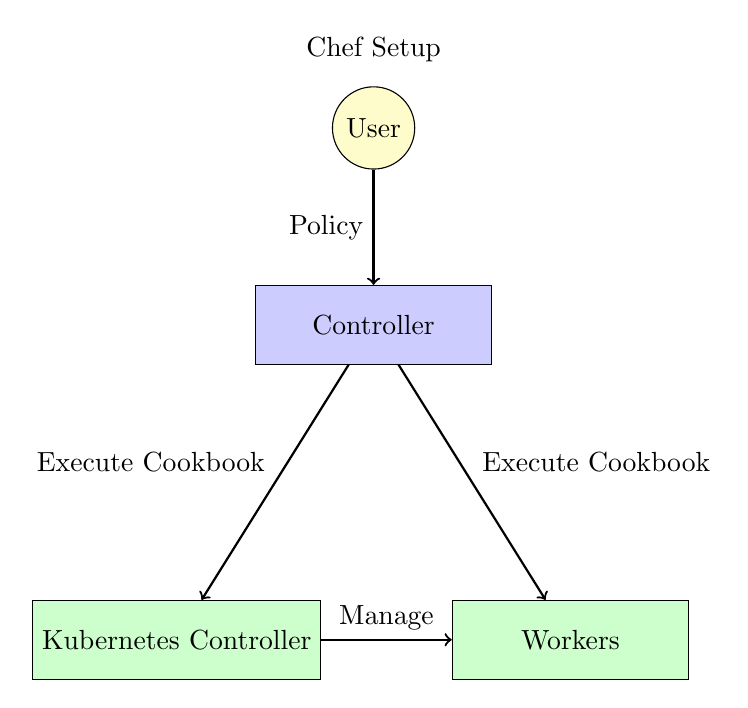
\begin{tikzpicture}
    
    % Draw the user
    \node[draw, circle, minimum size=1cm, fill=yellow!20] (user) at (0, 2.5) {User};
    
    % Draw the controller
    \node[draw, rectangle, minimum width=3cm, minimum height=1cm, fill=blue!20] (controller) at (0, 0) {Controller};
    
    % Draw the workers
    \node[draw, rectangle, minimum width=3cm, minimum height=1cm, fill=green!20] (worker1) at (-2.5, -4) {Kubernetes Controller};
    \node[draw, rectangle, minimum width=3cm, minimum height=1cm, fill=green!20] (workerN) at (2.5, -4) {Workers};
    
    % Draw connections
    \draw[->, thick] (user) -- node[midway, left] {Policy} (controller);
    \draw[->, thick] (controller) -- node[midway, above left] {Execute Cookbook} (worker1);
    \draw[->, thick] (controller) -- node[midway, above right] {Execute Cookbook} (workerN);
    \draw[->, thick] (worker1) --node[midway, above] {Manage} (workerN);
    % Optional: Add labels
    \node at (0, 3.5) {Chef Setup};
    % \node at (0, -5.5) {Executing Cookbooks};
    
    \end{tikzpicture}
    \caption{Example Chef Infrastructure}
    \label{fig:chef-infrastructure}
\end{figure}

% \subsection{Moving to a Bigger Scale}
% If the goal of the development would be 
% Local Development within an Ansible-Provisioned Machine and Migrating to the Cloud.





% Some of these were: different inventory.cfg needed for different local operating systems, some commands that could be executed locally displaying different behavior in the playbook, it being hard to update machine system configurations, limited verbosity in command outputs and very long wait times\cite{ansible-slow}. 

% At the end of the assignments, there is a complete local development environment. In this environment we can provision machines

% At the end of this project, we have a fairly complete local development environment. If this were a real-life situation, one would want to migrate the functionality we have created to an environment which a lot of people can use. 
